\begin{Schunk}
\begin{Sinput}
> library("Ham94", lib.loc = "../../../library")
\end{Sinput}
\end{Schunk}
January 1947 to November 1989, available in data source "indprod".  We will analyze the actual raw data, as well as
one month and one year log changes.
\begin{Schunk}
\begin{Sinput}
> data(indprod, package = "Ham94")
> selection <- subset(indprod, Month >= "1947-01-01" & Month <= 
+     "1989-11-01")
> raw.data <- selection$IPMFG6
> logdiff.data <- 100 * diff(log(raw.data), lag = 1)
> yeardiff.data <- 100 * diff(log(raw.data), lag = 12)
\end{Sinput}
\end{Schunk}
For plotting purposes, generate frequencies at regular intervals as show on page 159.  The first
spectrum uses unsmoothed estimates, the last two use a Bartlett kernel.
\begin{Schunk}
\begin{Sinput}
> s.Y.omega <- function(omega, gammas, params) {
+     1/(2 * pi) * (gammas[[1]] + 2 * as.numeric(t(gammas[-1]) %*% 
+         cos(1:(length(gammas) - 1) * omega)))
+ }
> s.Y.omega.Bartlett <- function(omega, gammas, params) {
+     1/(2 * pi) * (gammas[[1]] + 2 * as.numeric(t((1 - 1:params/(params + 
+         1)) * gammas[2:(params + 1)]) %*% cos(1:params * omega)))
+ }
> generate.plot.data <- function(values, estimator, params) {
+     T <- length(values)
+     acf.covariance <- acf(values, lag.max = T - 1, type = "covariance", 
+         plot = FALSE, demean = TRUE)
+     sapply(2 * pi/T * 1:((T - 1)/2), estimator, as.vector(acf.covariance$acf), 
+         params)
+ }
> raw.s.Y.omega <- generate.plot.data(raw.data, s.Y.omega, NULL)
> logdiff.s.Y.omega <- generate.plot.data(logdiff.data, s.Y.omega.Bartlett, 
+     12)
> yeardiff.s.Y.omega <- generate.plot.data(yeardiff.data, s.Y.omega.Bartlett, 
+     12)
\end{Sinput}
\end{Schunk}
The resulting output is shown below.
\begin{center}
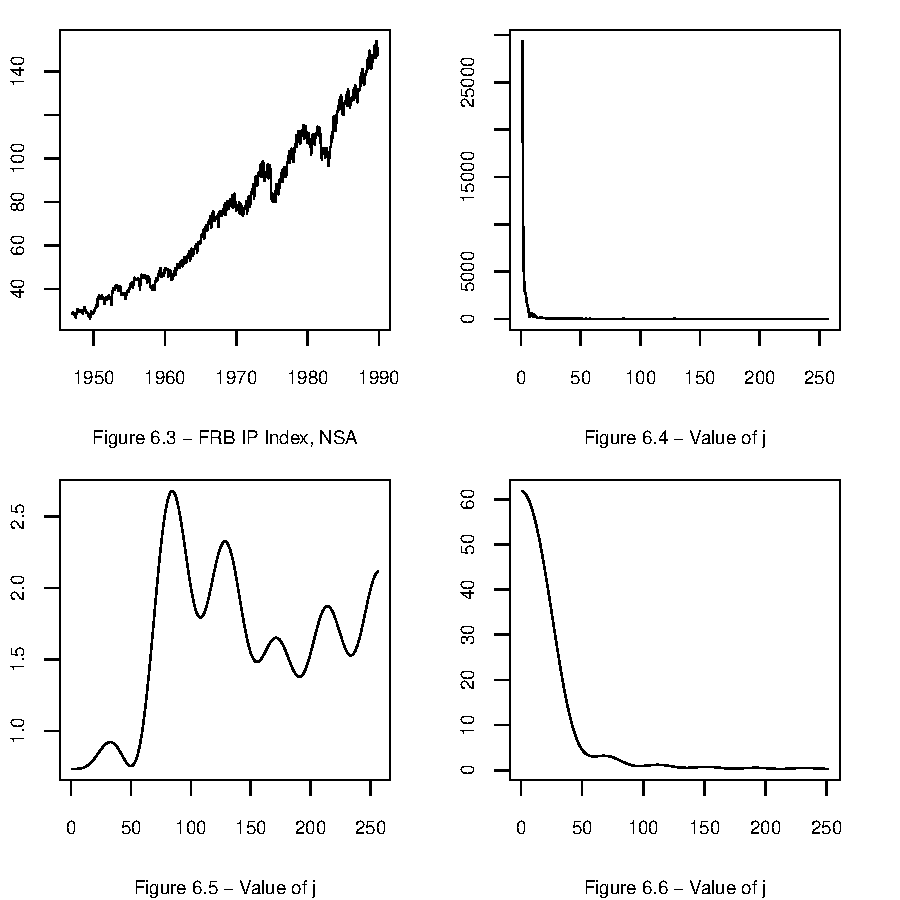
\includegraphics{p167-004}
\end{center}

